\section{Composite-Muster}

\subsection{Problemstellung}
Das Beispiel aus dem vorherigen Kapitel (Iteratoren) soll erweitert werden. 
\emph{Jetzt m"ochten sie eine Dessertkarte hinzuf"ugen. Gut. Und was jetzt? Jetzt m"ussen wir nicht nur mehrere Speisekarten, sondern auch noch Speisekarten in Speisekarten unterst"utzen. Es w"are sch"on, wenn wir die Dessertkarte einfach zu einem Element der Collection RestaurantSpeisekarte machen k"onnten, aber so wie das jetzt implementiert ist, funktioniert es nicht.}

\subsection{Erkl"arung des Musters}
\textbf{Definition}: Das Composite-Muster erm"oglicht es Ihnen, Objekte zu einer Baumstruktur zusammenzusetzen, um Teil/Ganzes-Hierarchien auszudr"ucken. Das Composite-Muster erlaubt den Clients, individuelle Objekte und Zusammensetzungen von Objekten auf gleiche Weise zu behandeln. 

\textbf{Wesentlicher Nachteil:} Alle Komponenten m"ussen die Schnittstelle Speisekarten-Komponente implementieren. Aber weil die Bl"atter und die Knoten unterschiedliche Rollen haben, k"onnen wir nicht f"ur alle Methoden eine sinnvolle Default-Implementierung definieren. Manchmal ist es noch dasd Beste, einfach eine Runtime-Exception auzul"osen. 

Das Iterieren innerhalb des Kompositum-Baums l"asst sich mithilfe eines neuen Iterators bewerkstelligen. Hierbei speichert jedes Element des Kompositums eine Liste von Iteratoren seiner Kindsknoten / Bl"atter. Dies wird rekursiv f"ur alle Kinder implementiert. Die Bl"atter bilden hierbei die Austrittsbedingung und geben einen Iterator zur"uck welcher lediglich "uber den Wert des eigenen Blattes iteriert. In den jeweils h"oheren Elementen wird zur Laufzeit dieser Stack von Element-Iteratoren nach und nach abgearbeitet. 


\paragraph{Punkt f"ur Punkt - S. 380}

\begin{itemize}[leftmargin=0.2in]
	\item Das Composite-Muster bietet eine Struktur, die einzelne Objekte und Komposita aufnehmen kann.
	\item Das Composite-Muster erlaubt Clients, Komposita und einzelne Objekte auf gleiche Weise zu behandeln. 
	\item Jede Objekt in einer zusammengesetzten Struktur ist eine Komponente. Komponenten k"onnen andere Komponenten oder Blattknoten sein. 
	\item Bei der Implementierung von Composite gibt es viele Designkompromisse. Sie m"ussen einen Ausgleich zwischen Transparenz und Sicherheit und Ihren Anforderungen finden.
\end{itemize}


\begin{figure}
	\centering
	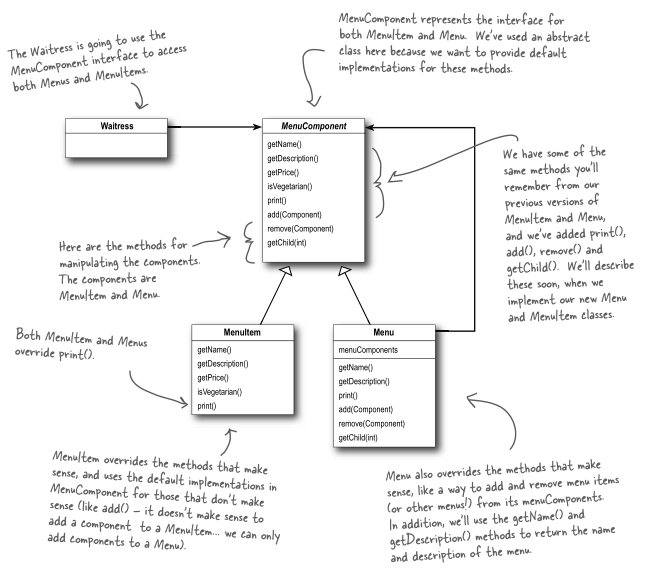
\includegraphics[width=.9\linewidth]{composite/img/compositeUML}
	\caption{UML-Darstellung des Composite-Musters}
	\label{fig:compositeUML}
\end{figure}
